\graphicspath{{content/chapters/5_evaluation/figures/}}

\chapter{Evaluation}%
\label{chp:evaluation}
\rule{\textwidth}{1pt} \\[1ex]

\epigraph{\textit{``It is not the strongest of the species that survive, nor the most intelligent, but the one most responsive to change.''}}{\textbf{-- Charles Darwin}}

\section{Introduction}
\label{sec:5_introduction}
% Grazzi Sinjur Alla, Ahfirli Sinjur Alla, u Ismaghni Sinjur Alla. Grazzi Amen

\section{Optimal Tiling Experiments}
\label{sec:5_tiling_exp}
% Glorja lil Missier, lil-Iben u lil- Ispirtu s-Santu, Kif kien fil bidu, issa u dejjem, ghal-dejjem. Amen
% all altitudes aggregated, since we require a detection model capable of generalising to different altitudes

%IMP Uncomment figures as you go along

% \begin{figure}[!ht]
%   \centering
%   \begin{tabular}{c}
%     \includegraphics[width=0.9\textwidth]{optimal_tiling_experiment_results_line1.png} \\
%     \small (a) \\
%     \addlinespace[1em]
%     \includegraphics[width=0.9\textwidth]{optimal_tiling_experiment_results_line2.png} \\
%     \small (b) \\
%   \end{tabular}
%   \caption{Optimal tiling experiment results on the \gls{soda} dataset, illustrating the increase in the number of images and annotated objects as the grid size increases. (a) Results over the full altitude range (1–30 metres), and (b) results on a subset of altitudes (5–30 metres) from the \gls{soda} dataset.}
%   \label{fig:optimal_tiling_line}
% \end{figure}

% \begin{figure}[!ht]
%   \centering
%   \begin{tabular}{c}
%     \includegraphics[width=0.9\textwidth]{optimal_tiling_experiment_elbow_method1.png} \\
%     \small (a) \\
%     \addlinespace[1em]
%     \includegraphics[width=0.9\textwidth]{optimal_tiling_experiment_elbow_method2.png} \\
%     \small (b) \\
%   \end{tabular}
%   \caption{Ratio of small objects to the number of images plotted against tiling grid size, highlighting the observed elbow point in red. (a) Results over the full altitude range (1–30 metres), and (b) results on a subset of altitudes (5–30 metres) from the \gls{soda} dataset.}
%   \label{fig:elbow_plot}
% \end{figure}


\section{Within-Dataset Evaluation}
\label{sec:5_within_dataset_exp}
% Grazzi Sinjur Alla, Ahfirli Sinjur Alla, u Ismaghni Sinjur Alla. Amen.

% N.B. Visual results and confusion matrix as well

\subsection{Binary Litter Detection on the SODA 1-metre Altitude Dataset}
\label{subsec:5_soda01m_dataset_exp}

% \begin{figure}[ht]
%     \centering
%     \includegraphics[width=1\textwidth]{SODA 01m Dataset (Single-label).png}
%     \caption{Comparison between the baseline and the best-performing student models across key detection metrics on the \gls{soda} dataset at a 1-metre altitude for binary litter detection.}
%     \label{fig:soda01m_bar}
% \end{figure}

% \begin{table}[ht]
%     \centering
%     \begin{adjustbox}{max width=\textwidth}
%     \renewcommand{\arraystretch}{1.5}
%     \begin{tabular}{|l|c|c|c|c|c|c|c|c|c|}
%         \hline%\toprule
%         \textbf{Model} & \textbf{mAP@50--95} & \textbf{mAP@50} & \textbf{mAP@75} & \textbf{mAR@1} & \textbf{mAR@10} & \textbf{mAR@100} & \textbf{Precision} & \textbf{Recall} & \textbf{F1 Score} \\ \hline \hline
%         \textbf{RetinaNet} & 0.94 & 0.98 & 0.96 & 0.63 & 0.96 & 0.96 & 0.93 & 0.99 & 0.96 \\\hline
%         \textbf{FCOS} & \textbf{0.96} & 0.98 & 0.97 & 0.63 & 0.97 & 0.97 & 0.81 & 0.99 & 0.89 \\\hline
%         \textbf{Faster R-CNN} & \textbf{0.96} & \textbf{0.99} & \textbf{0.98} & \textbf{0.63} & \textbf{0.98} & \textbf{0.98} & \textbf{0.99} & \textbf{0.99} & \textbf{0.99} \\\hline
%         \textbf{SSD} & 0.78 & 0.96 & 0.94 & 0.54 & 0.81 & 0.81 & 0.65 & 0.99 & 0.79 \\\hline
%         \textbf{SSDLite} & 0.61 & 0.73 & 0.72 & 0.48 & 0.63 & 0.63 & 0.02 & 0.99 & 0.03 \\
%         \hline%\bottomrule
%     \end{tabular}
%     \renewcommand{\arraystretch}{1}
%     \end{adjustbox}
%     \caption{Performance comparison of teacher models across key detection metrics, trained on the \gls{soda} dataset at a 1-metre altitude for binary litter detection.}
%     \label{tab:teacher_model_metrics_soda01m}
% \end{table}


% \begin{figure}[ht]
%     \centering
%     \includegraphics[width=1\textwidth]{training_times_soda_01m_dataset_binary_detection.png}
%     \caption{Comparison of model training times on the \gls{soda} dataset at a 1-metre altitude for binary litter detection.}
%     \label{fig:soda01m_training_time}
% \end{figure}

% \begin{table}[ht]
%     \centering
%     \begin{tabular}{llcc}
%         \toprule
%         \textbf{Model Configuration} & \textbf{Type} & \textbf{Size (MB)} & \textbf{Parameters (M)} \\
%         \midrule
%         \multirow{5}{*}{\textbf{Baseline}} 
%             & RetinaNet   & 122.72 & 32.17 \\
%             & FCOS        & 122.32 & 32.06 \\
%             & Faster R-CNN & 157.54 & 41.30 \\
%             & SSD         & 90.58  & 23.75 \\
%             & SSDLite     & 8.42   & 2.21 \\
%         \midrule
%         \multirow{5}{*}{\textbf{Student}} 
%             & RetinaNet   & 122.72 & 32.17 \\
%             & FCOS        & 122.32 & 32.06 \\
%             & Faster R-CNN & 157.54 & 41.30 \\
%             & SSD         & 90.58  & 23.75 \\
%             & SSSDLite     & 8.42   & 2.21 \\
%         \bottomrule
%     \end{tabular}
%     \caption{Comparison of model configurations for trained baseline and student models on the \gls{soda} dataset at a 1-metre altitude for binary litter detection, including model type, size in megabytes, and number of parameters (in millions).}
%     \label{tab:model_configs_soda01m}
% \end{table}


\subsection{Binary Litter Detection on the SODA All Altitudes Dataset}
\label{subsec:5_soda_tiled_single_dataset_exp}

% \begin{figure}[ht]
%     \centering
%     \includegraphics[width=1\textwidth]{SODA Dataset (Tiled Binary Detection).png}
%     \caption{Comparison between the baseline and best-performing student models across key detection metrics on the 3$\times$3 tiled \gls{soda} dataset across all altitudes for binary litter detection.}
%     \label{fig:soda_tiled_single_bar}
% \end{figure}

% \begin{table}[ht]
%     \centering
%     \begin{adjustbox}{max width=\textwidth}
%     \renewcommand{\arraystretch}{1.5}
%     \begin{tabular}{|l|c|c|c|c|c|c|c|c|c|}
%         \hline
%         \textbf{Model} & \textbf{mAP@50--95} & \textbf{mAP@50} & \textbf{mAP@75} & \textbf{mAR@1} & \textbf{mAR@10} & \textbf{mAR@100} & \textbf{Precision} & \textbf{Recall} & \textbf{F1 Score} \\ \hline \hline
%         \textbf{RetinaNet} & 0.90 & 0.95 & 0.94 & 0.34 & 0.83 & 0.91 & 0.41 & 0.98 & 0.58 \\\hline
%         \textbf{FCOS} & 0.89 & 0.94 & 0.93 & 0.34 & 0.82 & 0.90 & \textbf{0.97} & 0.96 & 0.96 \\\hline
%         \textbf{Faster R-CNN} & \textbf{0.96} & \textbf{0.99} & \textbf{0.98} & \textbf{0.35} & \textbf{0.87} & \textbf{0.97} & 0.96 & \textbf{0.99} & \textbf{0.98} \\\hline
%         \textbf{SSD} & 0.49 & 0.62 & 0.59 & 0.27 & 0.51 & 0.51 & 0.16 & 0.97 & 0.27 \\\hline
%         \textbf{SSDLite} & 0.18 & 0.23 & 0.19 & 0.17 & 0.19 & 0.19 & 0.00 & 0.79 & 0.01 \\
%         \hline
%     \end{tabular}
%     \renewcommand{\arraystretch}{1}
%     \end{adjustbox}
%     \caption{Performance comparison of teacher models across key detection metrics, trained on the 3$\times$3 tiled \gls{soda} dataset across all altitudes for binary litter detection.}
%     \label{tab:teacher_model_metrics_soda_tiled_single}
% \end{table}


% \begin{figure}[ht]
%     \centering
%     \includegraphics[width=1\textwidth]{training_times_soda_dataset_tiled_binary_detection.png}
%     \caption{Comparison of model training times on the 3$\times$3 tiled \gls{soda} dataset across all altitudes for binary litter detection.}
%     \label{fig:soda_tiled_single_training_time}
% \end{figure}

% \begin{table}[ht]
%     \centering
%     \begin{tabular}{llcc}
%         \toprule
%         \textbf{Model Configuration} & \textbf{Type} & \textbf{Size (MB)} & \textbf{Parameters (M)} \\
%         \midrule
%         \multirow{5}{*}{\textbf{Baseline}} 
%             & RetinaNet     & 122.72 & 32.17 \\
%             & FCOS          & 122.32 & 32.06 \\
%             & Faster R-CNN  & 157.54 & 41.30 \\
%             & SSD           & 90.58  & 23.75 \\
%             & SSDLite       & 8.42   & 2.21 \\
%         \midrule
%         \multirow{5}{*}{\textbf{Student}} 
%             & RetinaNet     & 122.72 & 32.17 \\
%             & FCOS          & 122.32 & 32.06 \\
%             & Faster R-CNN  & 157.54 & 41.30 \\
%             & SSD           & 90.58  & 23.75 \\
%             & SSDLite       & 8.42   & 2.21 \\
%         \bottomrule
%     \end{tabular}
%     \caption{Comparison of model configurations for trained baseline and student models on the 3$\times$3 tiled \gls{soda} dataset across all altitudes for binary litter detection, including model type, size in megabytes, and number of parameters (in millions).}
%     \label{tab:model_configs_soda_tiled_single}
% \end{table}


\subsection{Multi-label Litter Detection on the SODA All Altitudes Dataset}
\label{subsec:5_soda_tiled_multi_dataset_exp}

% \begin{figure}[ht]
%     \centering
%     \includegraphics[width=1\textwidth]{SODA Dataset (Tiled Multi-label Detection).png}
%     \caption{Comparison between the baseline and best-performing student models across key detection metrics on the 3$\times$3 tiled \gls{soda} dataset across all altitudes for multi-label litter detection.}
%     \label{fig:soda_tiled_multi_bar}
% \end{figure}

% \begin{table}[ht]
%     \centering
%     \begin{adjustbox}{max width=\textwidth}
%     \renewcommand{\arraystretch}{1.5}
%     \begin{tabular}{|l|c|c|c|c|c|c|c|c|c|}
%         \hline
%         \textbf{Model} & \textbf{mAP@50--95} & \textbf{mAP@50} & \textbf{mAP@75} & \textbf{mAR@1} & \textbf{mAR@10} & \textbf{mAR@100} & \textbf{Precision} & \textbf{Recall} & \textbf{F1 Score} \\ \hline \hline
%         \textbf{RetinaNet} & 0.88 & 0.92 & 0.91 & 0.66 & 0.89 & 0.89 & 0.76 & 0.97 & 0.85 \\\hline
%         \textbf{FCOS} & 0.91 & 0.95 & 0.94 & 0.68 & 0.92 & 0.92 & 0.91 & 0.97 & 0.94 \\\hline
%         \textbf{Faster R-CNN} & \textbf{0.95} & \textbf{0.99} & \textbf{0.98} & \textbf{0.70} & \textbf{0.96} & \textbf{0.96} & \textbf{0.96} & \textbf{0.99} & \textbf{0.97} \\\hline
%         \textbf{SSD} & 0.36 & 0.49 & 0.45 & 0.33 & 0.41 & 0.41 & 0.59 & 0.76 & 0.63 \\\hline
%         \textbf{SSDLite} & 0.11 & 0.13 & 0.13 & 0.13 & 0.13 & 0.13 & 0.00 & 0.37 & 0.01 \\
%         \hline
%     \end{tabular}
%     \renewcommand{\arraystretch}{1}
%     \end{adjustbox}
%     \caption{Performance comparison of teacher models across key detection metrics, trained on the 3$\times$3 tiled \gls{soda} dataset across all altitudes for multi-label litter detection.}
%     \label{tab:teacher_model_metrics_soda_tiled_multi}
% \end{table}


% \begin{figure}[ht]
%     \centering
%     \includegraphics[width=1\textwidth]{map_all_classes_soda_multi.png}
%     \caption{Comparison between the baseline and best-performing student models based on mean average precision by class on the 3$\times$3 tiled \gls{soda} dataset across all altitudes for multi-label litter detection.}
%     \label{fig:soda_tiled_multi_per_class}
% \end{figure}

% \begin{figure}[ht]
%   \centering
%   \begin{tabular}{cc}
%     \includegraphics[width=0.48\textwidth]{cm1.png} &
%     \includegraphics[width=0.48\textwidth]{cm2.png} \\
%     \small (a) & \small (b) \\
%   \end{tabular}
%   \caption{Normalised confusion matrices on the 3$\times$3 tiled \gls{soda} dataset across all altitudes for multi-label litter detection, using the best-performing models of the same architecture: (a) baseline, (b) student.}
%   \label{fig:cm_soda}
% \end{figure}

% \begin{figure}[ht]
%     \centering
%     \includegraphics[width=1\textwidth]{training_times_soda_dataset_tiled_multi_label_detection.png}
%     \caption{Comparison of model training times on 3$\times$3 tiled \gls{soda} dataset across all altitudes for multi-label litter detection.}
%     \label{fig:soda_tiled_multi_training_time}
% \end{figure}

% \begin{table}[ht]
%     \centering
%     \begin{tabular}{llcc}
%         \toprule
%         \textbf{Model Configuration} & \textbf{Type} & \textbf{Size (MB)} & \textbf{Parameters (M)} \\
%         \midrule
%         \multirow{5}{*}{\textbf{Baseline}} 
%             & RetinaNet     & 123.11 & 32.27 \\
%             & FCOS          & 122.36 & 32.08 \\
%             & Faster R-CNN  & 157.64 & 41.32 \\
%             & SSD           & 93.13  & 24.41 \\
%             & SSDLite       & 8.68   & 2.28 \\
%         \midrule
%         \multirow{5}{*}{\textbf{Student}} 
%             & RetinaNet     & 123.11 & 32.27 \\
%             & FCOS          & 122.36 & 32.08 \\
%             & Faster R-CNN  & 157.64 & 41.32 \\
%             & SSD           & 93.13  & 24.41 \\
%             & SSDLite       & 8.68   & 2.28 \\
%         \bottomrule
%     \end{tabular}
%     \caption{Comparison of model configurations for trained baseline and student models on the 3$\times$3 tiled \gls{soda} dataset across all altitudes for multi-label litter detection, including model type, size in megabytes, and number of parameters (in millions).}
%     \label{tab:model_configs_soda_tiled_multi}
% \end{table}


\subsection{Alpha Parameter Experiment}
\label{subsec:5_alpha_exp}

% \begin{figure}[ht]
%     \centering
%     \includegraphics[width=1\textwidth]{ablation_study_soda_01m.png}
%     \caption{Assessing the impact of the alpha (\gls{alpha}) parameter on student model performance, trained and evaluated on the \gls{soda} dataset at a 1-metre altitude for binary litter detection.}
%     \label{fig:ablation_soda01m}
% \end{figure}

% \begin{figure}[ht]
%     \centering
%     \includegraphics[width=1\textwidth]{ablation_study.png}
%     \caption{Assessing the impact of the alpha (\gls{alpha}) parameter on student model performance, trained and evaluated on the 3$\times$3 tiled \gls{soda} dataset across all altitudes for multi-label litter detection.}
%     \label{fig:ablation_soda_tiled_multi}
% \end{figure}

\section{Cross-Dataset Evaluation}
\label{sec:5_cross_dataset_exp}

\subsection{Binary Litter Detection on the BDW Dataset}
\label{subsec:5_bdw_exp}

% \begin{figure}[ht]
%     \centering
%     \includegraphics[width=1\textwidth]{BDW Dataset (Tested on Models Trained on SODA 01m Binary Detection).png}
%     \caption{Comparison of baseline and best-performing student models on key detection metrics using the \gls{bdw} dataset. The evaluated models were trained on the \gls{soda} dataset captured at 1-metre altitude for binary litter detection.}
%     \label{fig:bdw_bar}
% \end{figure}

\subsection{Binary Litter Detection on the UAVVaste Dataset}
\label{subsec:5_uavvaste_exp}

% \begin{figure}[ht]
%     \centering
%     \includegraphics[width=1\textwidth]{UAVVaste Dataset (Tested on Models Trained on SODA Tiled Binary Detection).png}
%     \caption{Comparison of baseline and best-performing student models on key detection metrics using the UAVVaste dataset. The evaluated models were trained on the 3$\times$3 tiled \gls{soda} dataset across all altitudes for binary litter detection.}
%     \label{fig:uavvaste_bar}
% \end{figure}

\section{Pascal VOC 2012 Evaluation}
\label{sec:5_pascal_voc_dataset_exp}

% \begin{figure}[ht]
%     \centering
%     \includegraphics[width=1\textwidth]{Pascal VOC 2012 Dataset (Multi-label Detection for 20 Classes) .png}
%     \caption{Comparison between the baseline and best-performing student models across key detection metrics on the Pascal VOC 2012 dataset for multi-label detection of 20 object classes.}
%     \label{fig:pascal_voc_bar}
% \end{figure}

% \begin{figure}[ht]
%     \centering
%     \includegraphics[width=1\textwidth]{map_all_classes_pascal_voc_no_text.png}
%     \caption{Comparison between the baseline and best-performing student models based on mean average precision by class on the Pascal VOC 2012 dataset for multi-label detection of 20 object classes.}
%     \label{fig:pascal_voc_per_class}
% \end{figure}

% \begin{table}[ht]
%     \centering
%     \begin{adjustbox}{max width=\textwidth}
%     \renewcommand{\arraystretch}{1.5}
%     \begin{tabular}{|l|c|c|c|c|c|c|c|c|c|}
%         \hline
%         \textbf{Model} & \textbf{mAP@50--95} & \textbf{mAP@50} & \textbf{mAP@75} & \textbf{mAR@1} & \textbf{mAR@10} & \textbf{mAR@100} & \textbf{Precision} & \textbf{Recall} & \textbf{F1 Score} \\ \hline \hline
%         \textbf{RetinaNet} & 0.77 & 0.86 & 0.79 & 0.60 & 0.81 & 0.81 & 0.26 & 0.90 & 0.38 \\\hline
%         \textbf{FCOS} & \textbf{0.80} & 0.88 & \textbf{0.82} & \textbf{0.61} & \textbf{0.84} & \textbf{0.84} & 0.43 & \textbf{0.91} & 0.56 \\\hline
%         \textbf{Faster R-CNN} & 0.77 & \textbf{0.91} & \textbf{0.82} & 0.59 & 0.82 & 0.82 & \textbf{0.56} & \textbf{0.91} & \textbf{0.68} \\\hline
%         \textbf{SSD} & 0.42 & 0.56 & 0.49 & 0.41 & 0.48 & 0.48 & 0.25 & 0.69 & 0.36 \\\hline
%         \textbf{SSDLite} & 0.49 & 0.61 & 0.54 & 0.46 & 0.55 & 0.55 & 0.04 & 0.79 & 0.07 \\
%         \hline
%     \end{tabular}
%     \renewcommand{\arraystretch}{1}
%     \end{adjustbox}
%     \caption{Performance comparison of teacher models across key detection metrics, trained on the Pascal VOC 2012 dataset for multi-label detection of 20 object classes.}
%     \label{tab:teacher_model_metrics_pascal_voc}
% \end{table}


% \begin{figure}[ht]
%     \centering
%     \includegraphics[width=1\textwidth]{training_times_pascal_voc_2012_dataset_multi_label_detection_for_20_classes.png}
%     \caption{Comparison of model training times on the Pascal VOC 2012 dataset for multi-label detection of 20 object classes.}
%     \label{fig:pascal_voc_training_time}
% \end{figure}

% \begin{figure}[ht]
%   \centering
%   \begin{tabular}{c}
%     \includegraphics[width=0.7\textwidth]{cm3.png} \\
%     \small (a) \\
%     \addlinespace[1em]
%     \includegraphics[width=0.7\textwidth]{cm4.png} \\
%      \small (b) \\
%   \end{tabular}
%   \caption{Normalised confusion matrices on the Pascal VOC 2012 dataset for multi-label detection of 20 object classes, using the best-performing models of the same architecture: (a) baseline, (b) student.}
%   \label{fig:cm_pascal_voc}
% \end{figure}

% \begin{table}[ht]
%     \centering
%     \begin{tabular}{llcc}
%         \toprule
%         \textbf{Model Configuration} & \textbf{Type} & \textbf{Size (MB)} & \textbf{Parameters (M)} \\
%         \midrule
%         \multirow{5}{*}{\textbf{Baseline}} 
%             & RetinaNet     & 124.22 & 32.56 \\
%             & FCOS          & 122.48 & 32.11 \\
%             & Faster R-CNN  & 157.92 & 41.40 \\
%             & SSD           & 100.27 & 26.29 \\
%             & SSDLite       & 9.42   & 2.47 \\
%         \midrule
%         \multirow{5}{*}{\textbf{Student}} 
%             & RetinaNet     & 124.22 & 32.56 \\
%             & FCOS          & 122.48 & 32.11 \\
%             & Faster R-CNN  & 157.92 & 41.40 \\
%             & SSD           & 100.27 & 26.29 \\
%             & SSDLite       & 9.42   & 2.47 \\
%         \bottomrule
%     \end{tabular}
%     \caption{Comparison of model configurations for trained baseline and student models on the Pascal VOC 2012 dataset for multi-label object detection, including model type, size in megabytes, and number of parameters (in millions).}
%     \label{tab:model_configs_pascal_voc}
% \end{table}


\section{Comparison of Visual Results and Model Interpretability}
\label{sec:5_interpretability}

% \begin{figure}[ht]
%   \centering
%   \begin{tabular}{cc}
%     \includegraphics[width=0.47\textwidth]{visual1.jpg} &
%     \includegraphics[width=0.47\textwidth]{visual2.jpg} \\
%     \small (a) & \small (b) \\
%     \addlinespace[1em]
%     \includegraphics[width=0.47\textwidth]{visual3.jpg} &
%     \includegraphics[width=0.47\textwidth]{visual4.jpg} \\
%     \small (c) & \small (d) \\
%   \end{tabular}
%   \caption{Comparison of predictions from the best-performing detection model trained on the \gls{soda} dataset. (a) and (c) show baseline model outputs, while (b) and (d) illustrate predictions from the corresponding student model.}
%   \label{fig:visuals_soda}
% \end{figure}

% \begin{figure}[ht]
%   \centering
%   \begin{tabular}{cc}
%     \includegraphics[width=0.47\textwidth]{visual5.jpg} &
%     \includegraphics[width=0.47\textwidth]{visual6.jpg} \\
%     \small (a) & \small (b) \\
%     \addlinespace[1em]
%     \includegraphics[width=0.47\textwidth]{visual7.jpg} &
%     \includegraphics[width=0.47\textwidth]{visual8.jpg} \\
%     \small (c) & \small (d) \\
%   \end{tabular}
%   \caption{Comparison of predictions from the best-performing detection model trained on the Pascal \gls{voc} 2012 dataset. (a) and (c) show baseline model outputs, while (b) and (d) illustrate predictions from the corresponding student model.}
%   \label{fig:visuals_pascal_voc}
% \end{figure}

% Grad CAM citations
% \begin{figure}[ht]
%     \centering
%     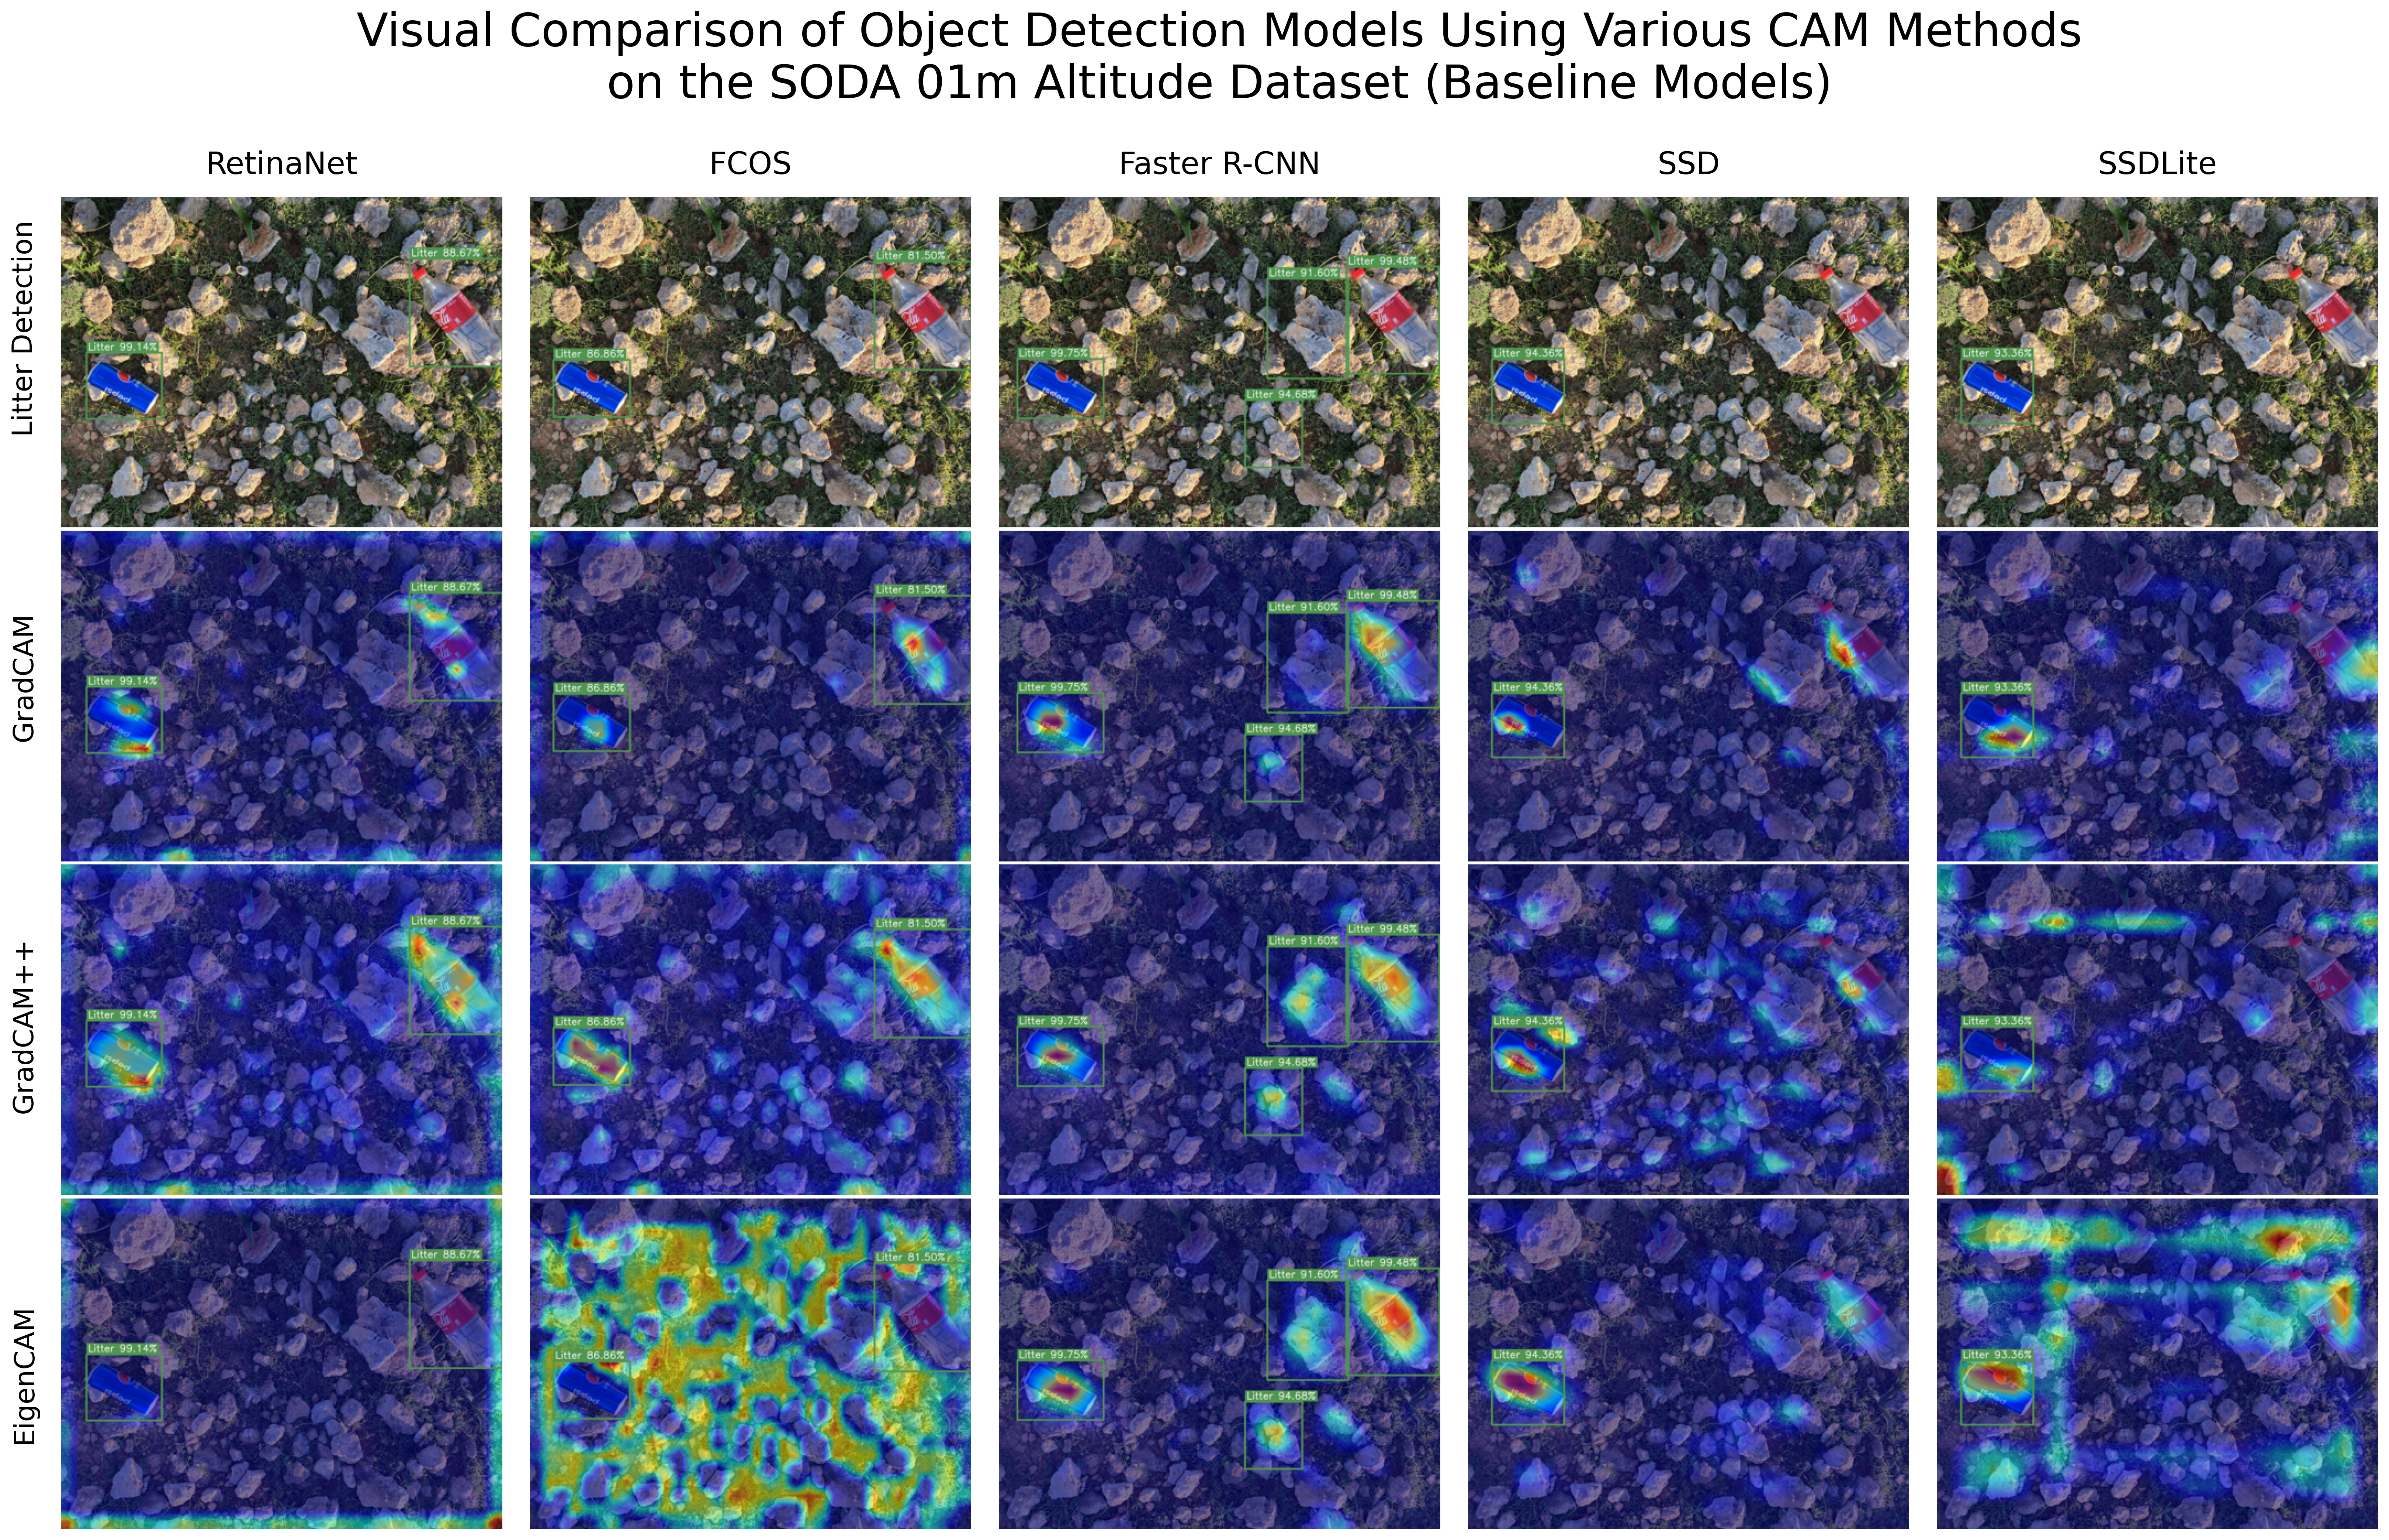
\includegraphics[width=1\textwidth]{gradcam_comparison_baseline.png}
%     \caption{Visual comparison of baseline object detection models using various \gls{cam} methods on the \gls{soda} dataset at a 1-metre altitude for binary litter detection.}
%     \label{fig:gradcam_baseline}
% \end{figure}

% \begin{figure}[ht]
%     \centering
%     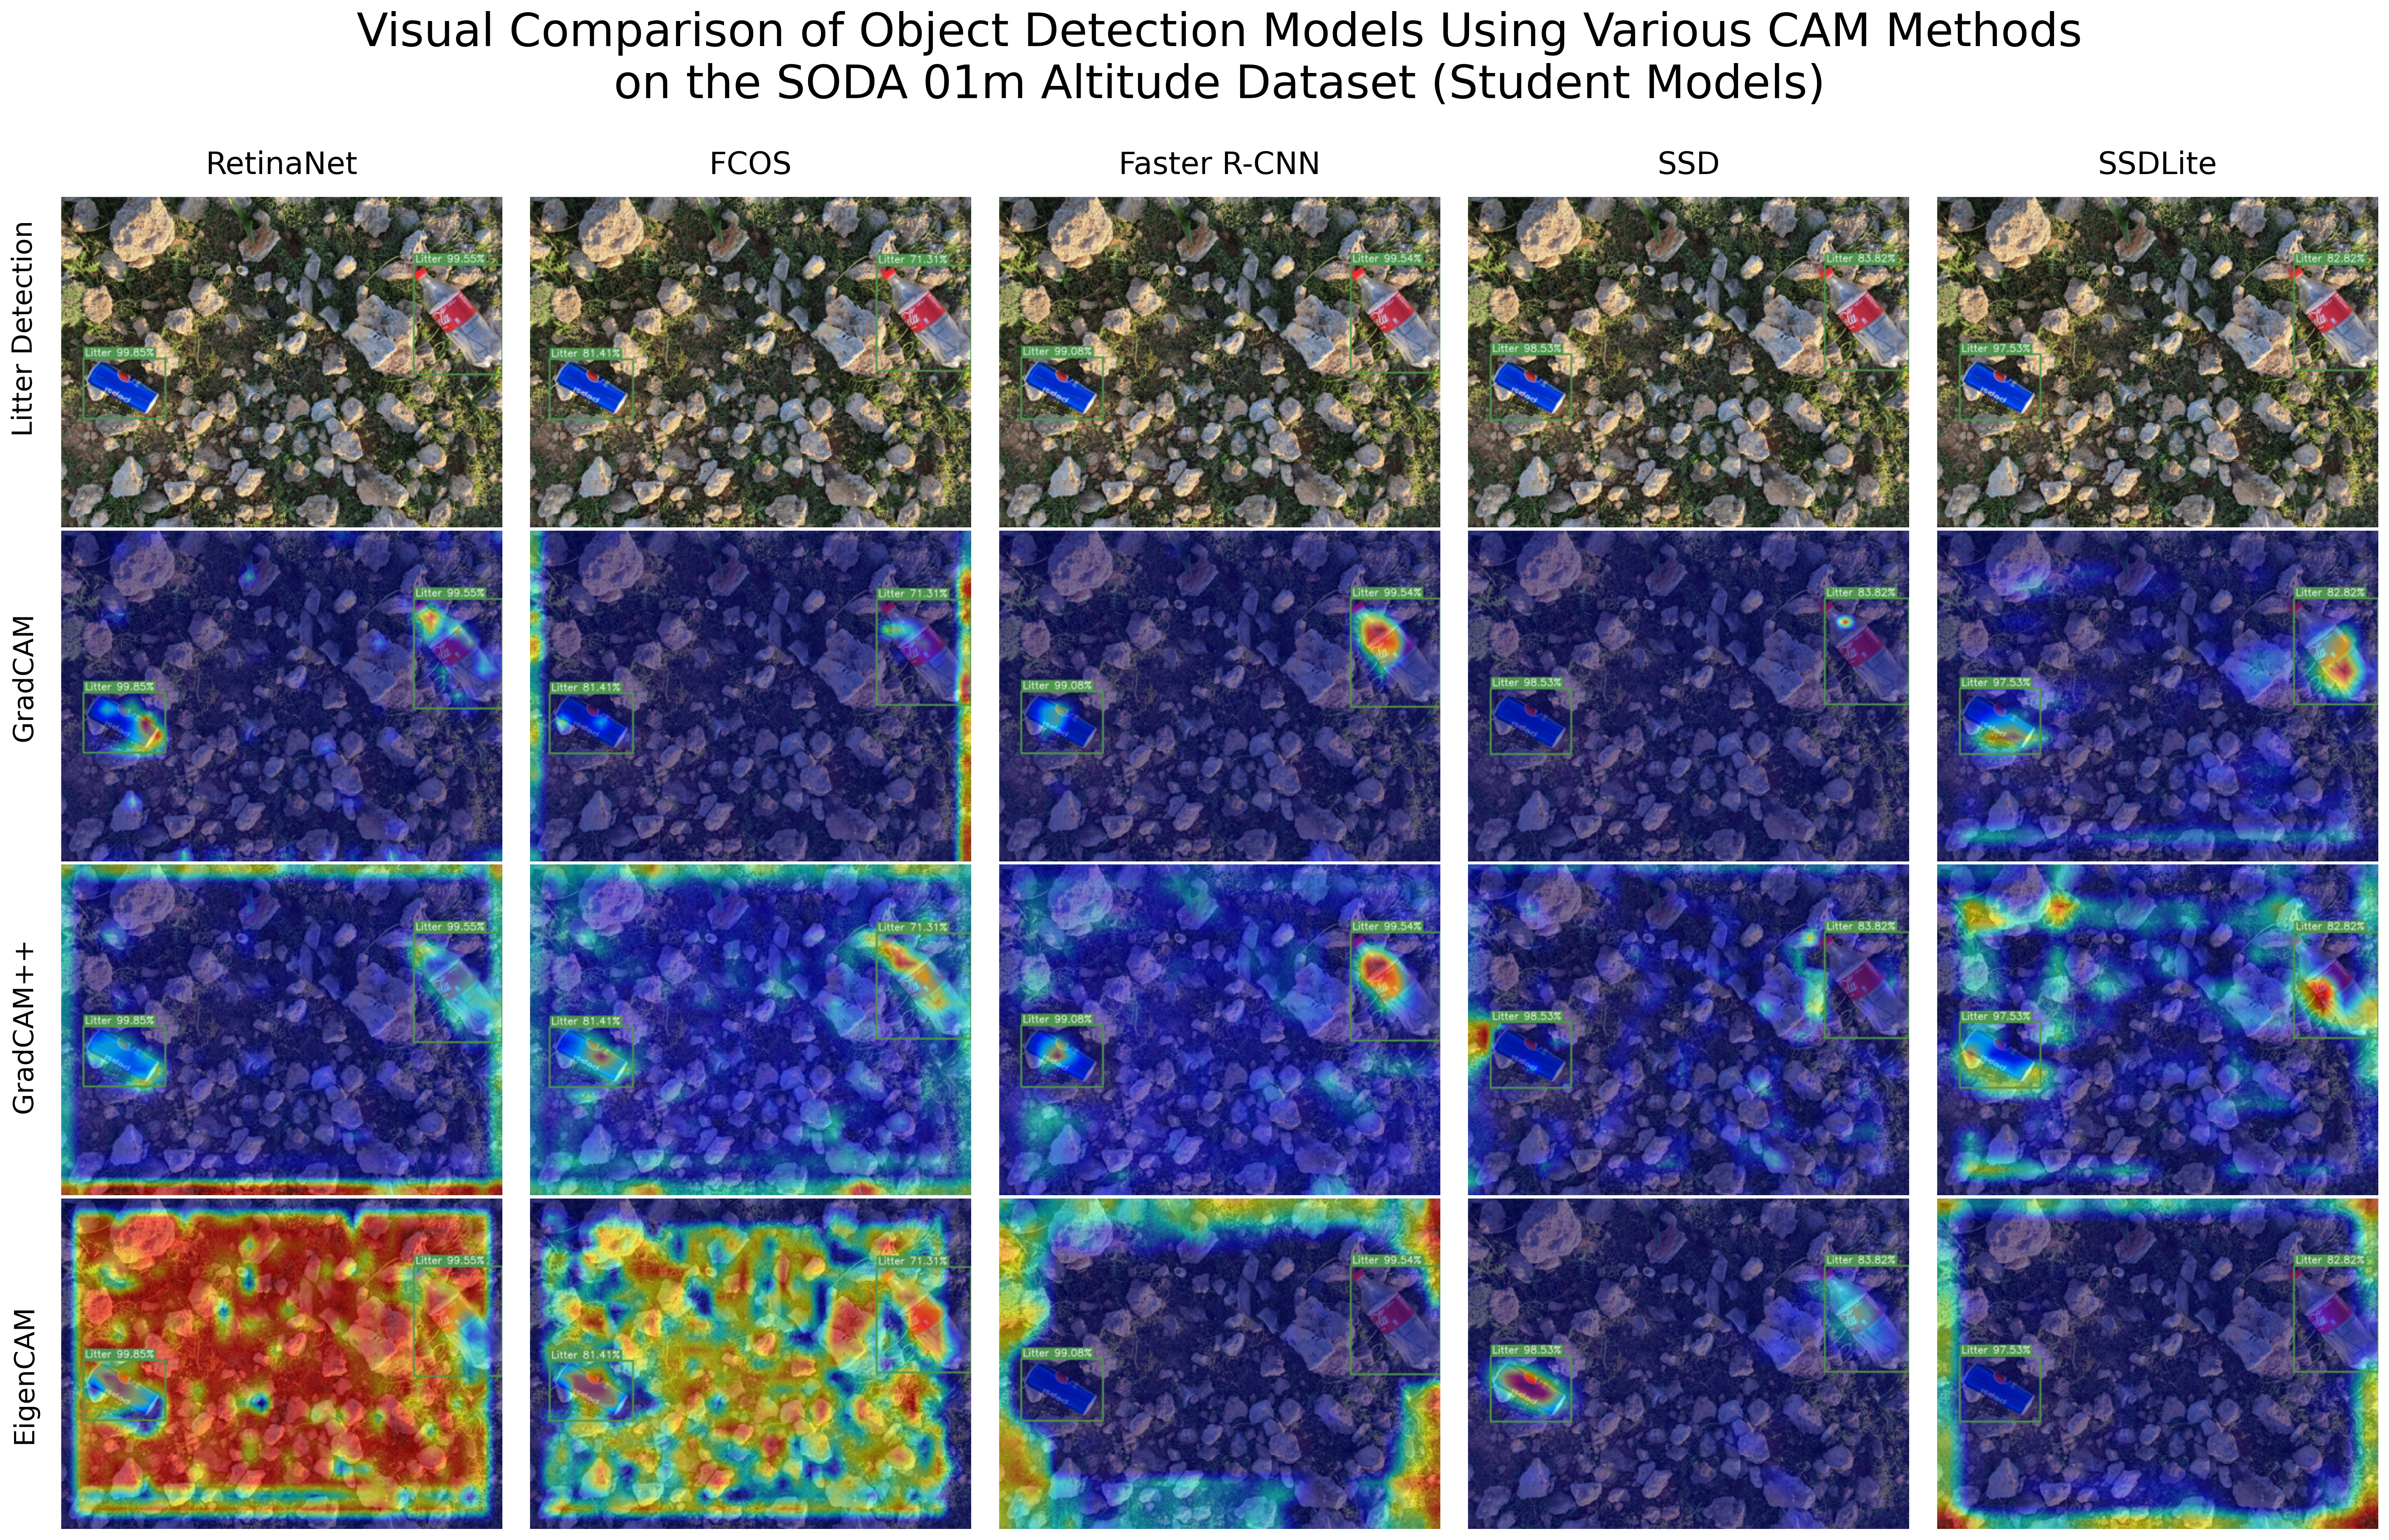
\includegraphics[width=1\textwidth]{gradcam_comparison_student.png}
%     \caption{Visual comparison of student object detection models using various \gls{cam} methods on the \gls{soda} dataset at a 1-metre altitude for binary litter detection.}
%     \label{fig:gradcam_student}
% \end{figure}

\section{Failure Cases in Privileged Information Generation}
\label{sec:5_fail_cases_priv_info_gen}

% \begin{figure}[ht]
%   \centering
%   \begin{tabular}{cc}
%     \includegraphics[width=0.48\textwidth]{fail_case1.jpg} &
%     \includegraphics[width=0.48\textwidth]{fail_case2.jpg} \\
%     \small (a) & \small (b) \\
%     \addlinespace[1em]
%     \includegraphics[width=0.48\textwidth]{fail_case3.jpg} &
%     \includegraphics[width=0.48\textwidth]{fail_case4.jpg} \\
%     \small (c) & \small (d) \\
%   \end{tabular}
%   \caption{Showcasing failure cases related to privileged information generation. (a) and (c) are original images from the Pascal VOC 2012 dataset, while (b) and (d) represent the corresponding privileged information.}
%   \label{fig:fail_cases}
% \end{figure}

\section{Discussion}
\label{sec:5_discussion}

\section{Conclusion}
\label{sec:5_conclusion}



%--

\begin{itemize}
    \item UREC Ethics Form - Done
    \item Problem Definition
    \item pages 110-120 maximum
    \item To check Daniel thesis
\end{itemize}

Evaluation
\begin{itemize}
    \item Tiling experiment - SODA include and exclude one meter magnification for SOD

    \item Experiment 1 - Within dataset evaluation
    \item Within dataset - 3 tas SODA Dataset - show all charts and tables + discussion
    \item Ablation studies - alpha for LUPI and Distillation (nest inside)
    \item Across dataset - BDW and UAVVaste
    \item Generalisation - Pascal VOC
    \item Visual Analysis, Ground truth, mask overlap, litter predictions
    \item Interpretability Grad CAM
    \item Discussion - Go over research question once more, theoretical aspect, Knowledge Distillation and Applications - Project AWIGS, summary
\end{itemize}

Conclusion
Revisting aims and objectives
limitation and future work (everything from future work goes here)
Conclusion

Future Work - Future Research/Future Projects
\begin{itemize}
    \item Trying out this method for Segmentation
    \item generalisation capabilities on Pascal VOC and COCO to ask what to include
    \item Test out the method on state-of-the art object deteciton architectures such as YOLO11 etc. . . - can be a limitation
    \item considerations of real time or alternatives to privileged information
    \item Improvement in terms of encoding the bounding boxes for the teacher better and iinvestigating in better channels etc. . . (to ask)
    \item further tests on generalisation of higher class datasets and training parameters
\end{itemize}

%--
